\documentclass[a4paper]{article}

\usepackage[english]{babel}
\usepackage[utf8]{inputenc}
\usepackage{amsmath}
\usepackage{graphicx}
\usepackage[colorinlistoftodos]{todonotes}
\usepackage[export]{adjustbox}[2011/08/13]
\usepackage{float}
\usepackage{bm}

\title{Behaviour Dynamics in Social Networks - Assignment 4}

\author{Maria Hotoiu, Federico Tavella}

\date{\today}

\begin{document}
\maketitle

\begin{abstract}
Learn to use parameter tuning tools to find the best values for a set of missing parameter values in a model.
\end{abstract}

\section{Part 1}

\begin{figure}[!htpb]
\center
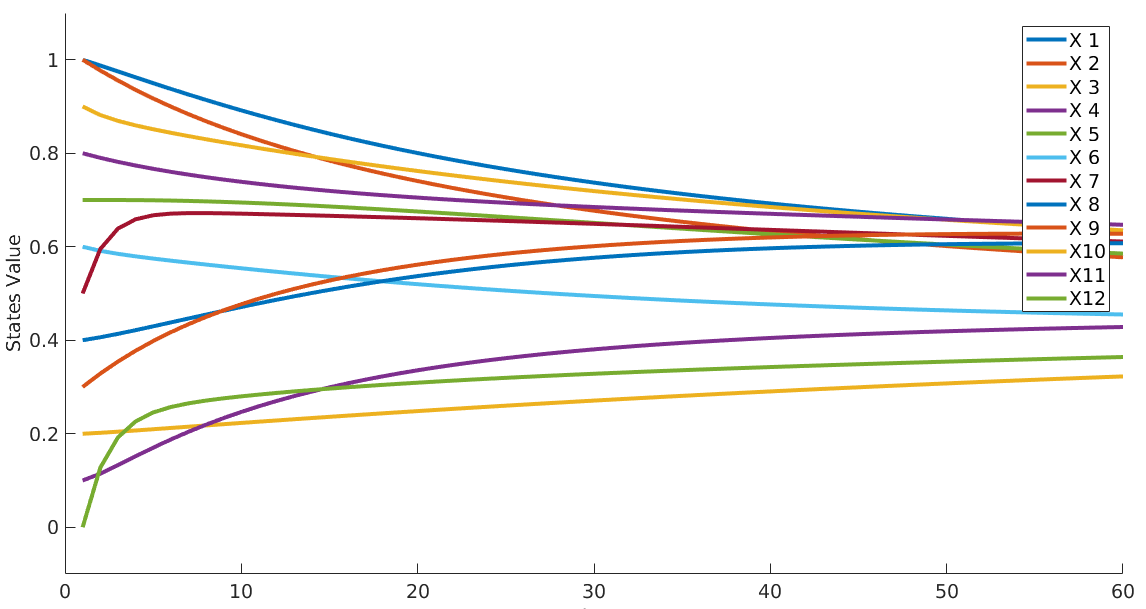
\includegraphics[width=\textwidth]{res/img/part1}
\caption{Results from the simulation}
\label{fig:part1}
\end{figure}

\section{Part 2}


\begin{table}[H]
\centering
\begin{adjustbox}{width=1.2\textwidth,center=\textwidth}
\begin{tabular}{c|c|c|c|c|c|c|c}
\bm{$\eta_{L}$} & \textbf{K(t = 2)} & \textbf{L(t = 2)} & \textbf{$|$K-L(t = 2)$|$} & \textbf{K(t = 13)} & \textbf{L(t = 13)} & \textbf{$|$K-L(t = 13)$|$} & \textbf{Sum of differences} \\ \hline
0                   & 0.1146            & 0                 & 0.1146                    & 0.2221             & 0                  & 0.2221                     & 0.3367                      \\
0.05                & 0.1146            & 0.0127            & 0.1019                    & 0.2395             & 0.1232             & 0.1162                     & 0.2181                      \\
0.10                & 0.1146            & 0.0255            & 0.0892                    & 0.2517             & 0.1949             & 0.0568                     & 0.1460                      \\
0.15                & 0.1146            & 0.0382            & 0.0765                    & 0.2603             & 0.2359             & 0.0243                     & 0.1008                      \\
0.20                & 0.1146            & 0.0509            & 0.0637                    & 0.2664             & 0.2592             & 0.0072                     & 0.0709                      \\
0.25                & 0.1146            & 0.0636            & 0.0510                    & 0.2708             & 0.2724             & 0.0016                     & 0.0526                      \\
0.30                & 0.1146            & 0.0764            & 0.0383                    & 0.2739             & 0.2799             & 0.0060                     & 0.0443                      \\
0.35                & 0.1146            & 0.0891            & 0.0256                    & 0.2763             & 0.2844             & 0.0081                     & 0.0337                      \\
0.40                & 0.1146            & 0.1018            & 0.0128                    & 0.2781             & 0.2873             & 0.0092                     & 0.0220                      \\
0.45                & 0.1146            & 0.1145            & 0.0001                    & 0.2795             & 0.2892             & 0.0097                     & 0.0098                      \\
0.50                & 0.1146            & 0.1273            & 0.0126                    & 0.2806             & 0.2906             & 0.0100                     & 0.0226                     
\end{tabular}
\end{adjustbox}
\caption{Exhaustive search for different values of $\eta_{L}$}
\label{tab:exaustive_search}
\end{table}

The best value for $\eta_{L}$ (i.e. the one with the minimum sum of differences at $t = 2$ and $t = 13$) is $\eta_{L} = 0.45$.

\begin{figure}[!htpb]
\center
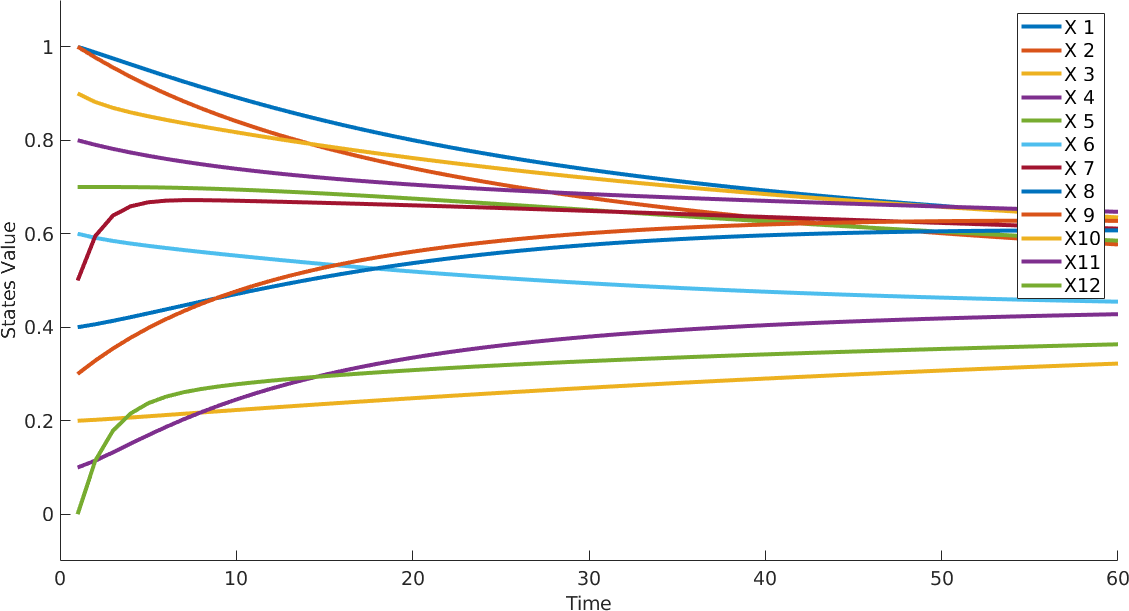
\includegraphics[width=\textwidth]{res/img/exhaustive_search_part2}
\caption{Results from the simulation for $\eta_{L} = 0.45$}
\label{fig:exhaustive_search_part2}
\end{figure}

\section{Part 3}

\begin{table}[H]
\centering
\begin{tabular}{c|c|c}
\bm{$\eta_{L}$} & \textbf{SSR} & \textbf{Error}\\ \hline
                                        
                                   
0 & 0.9593 & 0.2827  \\                                       
0.05 & 0.0222 &   0.0430   \\
0.10  & 0.0463  & 0.0621 \\
0.15  &  0.1618 & 0.1161  \\  
0.20  & 0.2621   &  0.1478 \\
0.25 & 0.3402 &  0.1684\\
0.30 & 0.4010 &  0.1828  \\
0.35 & 0.4491  &  0.1935  \\ 
0.40  & 0.4881 & 0.2017 \\
0.45  & 0.5202 &  0.2082\\
0.50 &  0.5472 & 0.2135                                                                                                              
\end{tabular}
\caption{Exhaustive search for different values of $\eta_{L}$}
\label{tab:exaustive_searchSSR}
\end{table}

The best value for $\eta_{L}$ is $\eta_{L} = 0.05$. In Figure~\ref{fig:part3}, we can see how the error derived from the simulation is of the same magnitude of the one represented in the graph.

\begin{figure}[!h]
\center
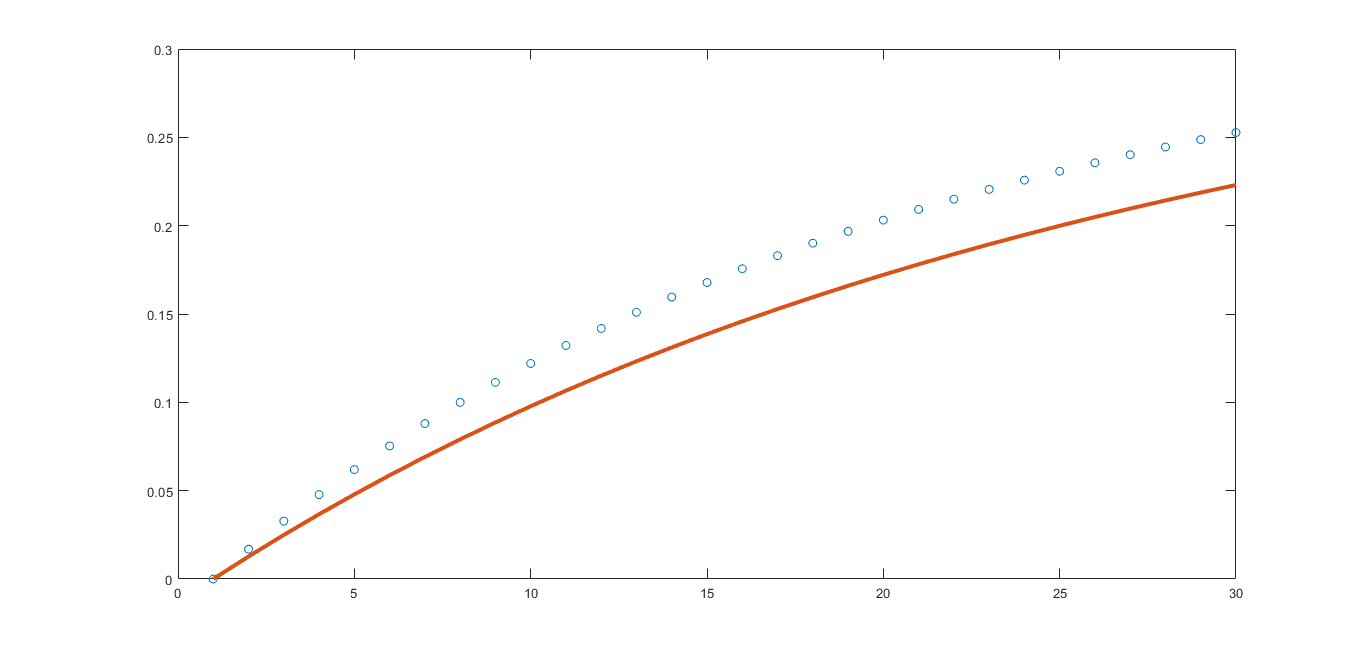
\includegraphics[width=\textwidth]{res/img/plotdiff}
\caption{Simulated values for  $\eta_{L} = 0.05$ (line) vs empirical values (dots)}
\label{fig:part3}
\end{figure}

\newpage

\section{Part 4}

If we want to use exhaustive search with grain size of 0.01, we should check $101^{12}$ sets of values.

\begin{table}[H]
\centering
\begin{tabular}{c|c}
\bm{$\eta_{i}$} & \textbf{Value} \\ \hline
                            
$\eta_{1}$ & 0.257 \\                                       
$\eta_{2}$ & 0.105 \\ 
$\eta_{3}$ & 0.062 \\ 
$\eta_{4}$ & 0.078 \\ 
$\eta_{5}$ & 0.323 \\ 
$\eta_{6}$ & 0.089 \\ 
$\eta_{7}$ & 0.370 \\ 
$\eta_{8}$ & 0.229 \\ 
$\eta_{9}$ & 0.113 \\ 
$\eta_{10}$ & 0.032 \\ 
$\eta_{11}$ & 0.139 \\ 
$\eta_{12}$ & 0.312 \\ 

\end{tabular}
\caption{Best set of values for $\eta$ }
\label{tab:exaustive_search_eta}
\end{table}

The error corresponding to these speed factors is 0.1046. It is worth to mention that, due to randomicity in the Simulated Annealing algorithm, two different run of the optimization tool will rarely lead to the same values - thus, to the same corresponding error.

\begin{figure}[H]
\center
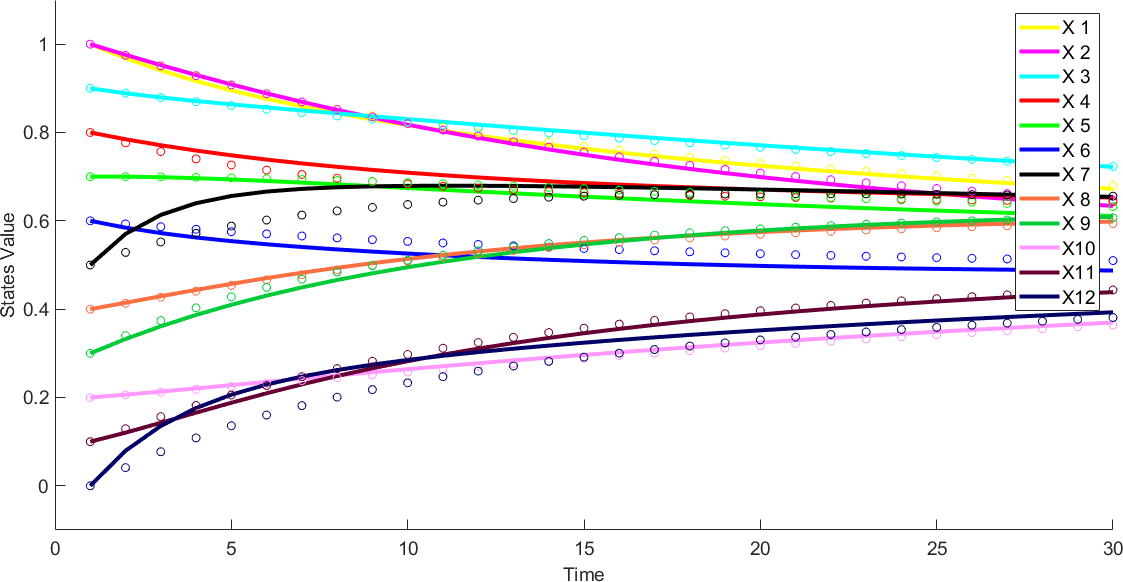
\includegraphics[width=\textwidth]{res/img/plotdiff2}
\caption{Simulated values vs empirical values }
\label{fig:plotdiff2}
\end{figure}

\end{document}
